% Created by tikzDevice version 0.12.6 on 2024-01-02 14:56:37
% !TEX encoding = UTF-8 Unicode
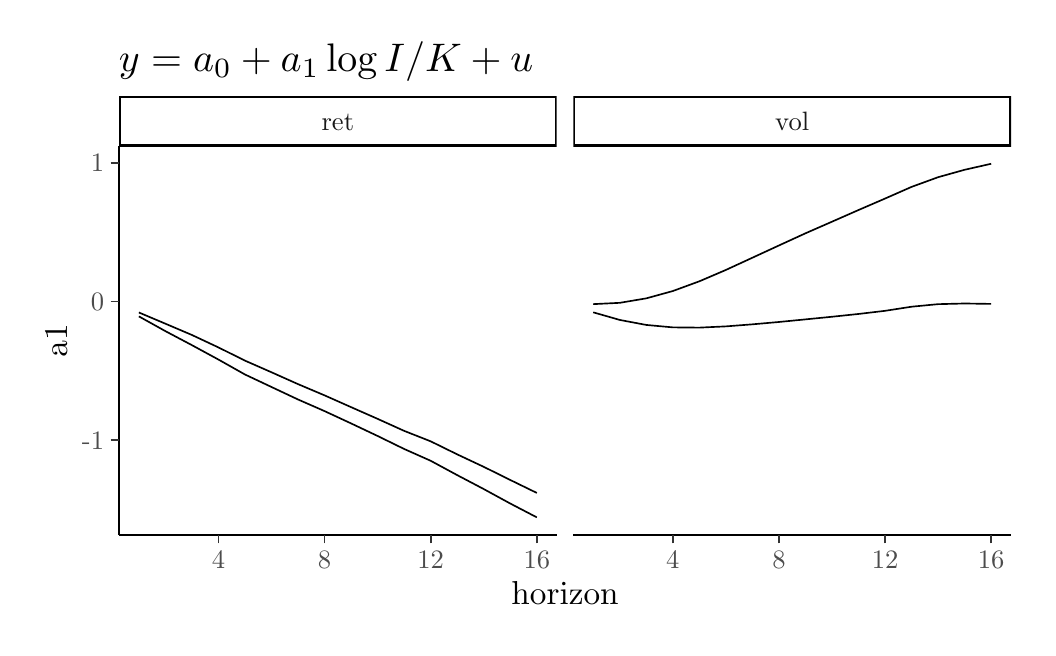
\begin{tikzpicture}[x=1pt,y=1pt]
\definecolor{fillColor}{RGB}{255,255,255}
\path[use as bounding box,fill=fillColor,fill opacity=0.00] (0,0) rectangle (361.35,216.81);
\begin{scope}
\path[clip] (  0.00,  0.00) rectangle (361.35,216.81);
\definecolor{drawColor}{RGB}{255,255,255}
\definecolor{fillColor}{RGB}{255,255,255}

\path[draw=drawColor,line width= 0.6pt,line join=round,line cap=round,fill=fillColor] (  0.00,  0.00) rectangle (361.35,216.81);
\end{scope}
\begin{scope}
\path[clip] ( 33.00, 33.48) rectangle (191.17,174.02);
\definecolor{fillColor}{RGB}{255,255,255}

\path[fill=fillColor] ( 33.00, 33.48) rectangle (191.17,174.02);
\definecolor{drawColor}{RGB}{0,0,0}

\path[draw=drawColor,line width= 0.6pt,line join=round] ( 40.19,113.89) --
	( 49.77,109.84) --
	( 59.36,105.76) --
	( 68.94,101.26) --
	( 78.53, 96.49) --
	( 88.12, 92.28) --
	( 97.70, 88.00) --
	(107.29, 83.94) --
	(116.88, 79.68) --
	(126.46, 75.45) --
	(136.05, 71.11) --
	(145.64, 67.33) --
	(155.22, 62.62) --
	(164.81, 58.11) --
	(174.40, 53.36) --
	(183.98, 48.69);

\path[draw=drawColor,line width= 0.6pt,line join=round] ( 40.19,112.48) --
	( 49.77,107.15) --
	( 59.36,102.08) --
	( 68.94, 96.88) --
	( 78.53, 91.48) --
	( 88.12, 86.96) --
	( 97.70, 82.45) --
	(107.29, 78.25) --
	(116.88, 73.80) --
	(126.46, 69.26) --
	(136.05, 64.57) --
	(145.64, 60.30) --
	(155.22, 55.12) --
	(164.81, 50.08) --
	(174.40, 44.85) --
	(183.98, 39.86);
\end{scope}
\begin{scope}
\path[clip] (197.17, 33.48) rectangle (355.35,174.02);
\definecolor{fillColor}{RGB}{255,255,255}

\path[fill=fillColor] (197.17, 33.48) rectangle (355.35,174.02);
\definecolor{drawColor}{RGB}{0,0,0}

\path[draw=drawColor,line width= 0.6pt,line join=round] (204.36,113.95) --
	(213.95,111.20) --
	(223.54,109.39) --
	(233.12,108.51) --
	(242.71,108.42) --
	(252.30,108.87) --
	(261.88,109.61) --
	(271.47,110.46) --
	(281.05,111.40) --
	(290.64,112.35) --
	(300.23,113.36) --
	(309.81,114.49) --
	(319.40,115.98) --
	(328.99,116.90) --
	(338.57,117.14) --
	(348.16,116.99);

\path[draw=drawColor,line width= 0.6pt,line join=round] (204.36,116.91) --
	(213.95,117.38) --
	(223.54,119.00) --
	(233.12,121.64) --
	(242.71,125.16) --
	(252.30,129.27) --
	(261.88,133.68) --
	(271.47,138.11) --
	(281.05,142.50) --
	(290.64,146.70) --
	(300.23,150.92) --
	(309.81,155.06) --
	(319.40,159.28) --
	(328.99,162.78) --
	(338.57,165.46) --
	(348.16,167.63);
\end{scope}
\begin{scope}
\path[clip] ( 33.00,174.02) rectangle (191.17,192.09);
\definecolor{drawColor}{RGB}{0,0,0}
\definecolor{fillColor}{RGB}{255,255,255}

\path[draw=drawColor,line width= 1.2pt,line join=round,line cap=round,fill=fillColor] ( 33.00,174.02) rectangle (191.17,192.09);
\definecolor{drawColor}{gray}{0.10}

\node[text=drawColor,anchor=base,inner sep=0pt, outer sep=0pt, scale=  0.96] at (112.08,179.75) {ret};
\end{scope}
\begin{scope}
\path[clip] (197.17,174.02) rectangle (355.35,192.09);
\definecolor{drawColor}{RGB}{0,0,0}
\definecolor{fillColor}{RGB}{255,255,255}

\path[draw=drawColor,line width= 1.2pt,line join=round,line cap=round,fill=fillColor] (197.17,174.02) rectangle (355.35,192.09);
\definecolor{drawColor}{gray}{0.10}

\node[text=drawColor,anchor=base,inner sep=0pt, outer sep=0pt, scale=  0.96] at (276.26,179.75) {vol};
\end{scope}
\begin{scope}
\path[clip] (  0.00,  0.00) rectangle (361.35,216.81);
\definecolor{drawColor}{RGB}{0,0,0}

\path[draw=drawColor,line width= 0.6pt,line join=round] ( 33.00, 33.48) --
	(191.17, 33.48);
\end{scope}
\begin{scope}
\path[clip] (  0.00,  0.00) rectangle (361.35,216.81);
\definecolor{drawColor}{gray}{0.20}

\path[draw=drawColor,line width= 0.6pt,line join=round] ( 68.94, 30.48) --
	( 68.94, 33.48);

\path[draw=drawColor,line width= 0.6pt,line join=round] (107.29, 30.48) --
	(107.29, 33.48);

\path[draw=drawColor,line width= 0.6pt,line join=round] (145.64, 30.48) --
	(145.64, 33.48);

\path[draw=drawColor,line width= 0.6pt,line join=round] (183.98, 30.48) --
	(183.98, 33.48);
\end{scope}
\begin{scope}
\path[clip] (  0.00,  0.00) rectangle (361.35,216.81);
\definecolor{drawColor}{gray}{0.30}

\node[text=drawColor,anchor=base,inner sep=0pt, outer sep=0pt, scale=  0.96] at ( 68.94, 21.46) {4};

\node[text=drawColor,anchor=base,inner sep=0pt, outer sep=0pt, scale=  0.96] at (107.29, 21.46) {8};

\node[text=drawColor,anchor=base,inner sep=0pt, outer sep=0pt, scale=  0.96] at (145.64, 21.46) {12};

\node[text=drawColor,anchor=base,inner sep=0pt, outer sep=0pt, scale=  0.96] at (183.98, 21.46) {16};
\end{scope}
\begin{scope}
\path[clip] (  0.00,  0.00) rectangle (361.35,216.81);
\definecolor{drawColor}{RGB}{0,0,0}

\path[draw=drawColor,line width= 0.6pt,line join=round] (197.17, 33.48) --
	(355.35, 33.48);
\end{scope}
\begin{scope}
\path[clip] (  0.00,  0.00) rectangle (361.35,216.81);
\definecolor{drawColor}{gray}{0.20}

\path[draw=drawColor,line width= 0.6pt,line join=round] (233.12, 30.48) --
	(233.12, 33.48);

\path[draw=drawColor,line width= 0.6pt,line join=round] (271.47, 30.48) --
	(271.47, 33.48);

\path[draw=drawColor,line width= 0.6pt,line join=round] (309.81, 30.48) --
	(309.81, 33.48);

\path[draw=drawColor,line width= 0.6pt,line join=round] (348.16, 30.48) --
	(348.16, 33.48);
\end{scope}
\begin{scope}
\path[clip] (  0.00,  0.00) rectangle (361.35,216.81);
\definecolor{drawColor}{gray}{0.30}

\node[text=drawColor,anchor=base,inner sep=0pt, outer sep=0pt, scale=  0.96] at (233.12, 21.46) {4};

\node[text=drawColor,anchor=base,inner sep=0pt, outer sep=0pt, scale=  0.96] at (271.47, 21.46) {8};

\node[text=drawColor,anchor=base,inner sep=0pt, outer sep=0pt, scale=  0.96] at (309.81, 21.46) {12};

\node[text=drawColor,anchor=base,inner sep=0pt, outer sep=0pt, scale=  0.96] at (348.16, 21.46) {16};
\end{scope}
\begin{scope}
\path[clip] (  0.00,  0.00) rectangle (361.35,216.81);
\definecolor{drawColor}{RGB}{0,0,0}

\path[draw=drawColor,line width= 0.6pt,line join=round] ( 33.00, 33.48) --
	( 33.00,174.02);
\end{scope}
\begin{scope}
\path[clip] (  0.00,  0.00) rectangle (361.35,216.81);
\definecolor{drawColor}{gray}{0.30}

\node[text=drawColor,anchor=base east,inner sep=0pt, outer sep=0pt, scale=  0.96] at ( 27.60, 64.40) {-1};

\node[text=drawColor,anchor=base east,inner sep=0pt, outer sep=0pt, scale=  0.96] at ( 27.60,114.54) {0};

\node[text=drawColor,anchor=base east,inner sep=0pt, outer sep=0pt, scale=  0.96] at ( 27.60,164.68) {1};
\end{scope}
\begin{scope}
\path[clip] (  0.00,  0.00) rectangle (361.35,216.81);
\definecolor{drawColor}{gray}{0.20}

\path[draw=drawColor,line width= 0.6pt,line join=round] ( 30.00, 67.71) --
	( 33.00, 67.71);

\path[draw=drawColor,line width= 0.6pt,line join=round] ( 30.00,117.85) --
	( 33.00,117.85);

\path[draw=drawColor,line width= 0.6pt,line join=round] ( 30.00,167.99) --
	( 33.00,167.99);
\end{scope}
\begin{scope}
\path[clip] (  0.00,  0.00) rectangle (361.35,216.81);
\definecolor{drawColor}{RGB}{0,0,0}

\node[text=drawColor,anchor=base,inner sep=0pt, outer sep=0pt, scale=  1.20] at (194.17,  8.33) {horizon};
\end{scope}
\begin{scope}
\path[clip] (  0.00,  0.00) rectangle (361.35,216.81);
\definecolor{drawColor}{RGB}{0,0,0}

\node[text=drawColor,rotate= 90.00,anchor=base,inner sep=0pt, outer sep=0pt, scale=  1.20] at ( 14.26,103.75) {a1};
\end{scope}
\begin{scope}
\path[clip] (  0.00,  0.00) rectangle (361.35,216.81);
\definecolor{drawColor}{RGB}{0,0,0}

\node[text=drawColor,anchor=base west,inner sep=0pt, outer sep=0pt, scale=  1.44] at ( 33.00,200.89) {$y = a_0 + a_1 \log I/K +u$};
\end{scope}
\end{tikzpicture}
